\documentclass[12pt,a4paper]{article}

% ─── Page Layout ───────────────────────────────────────────────────────────────
\usepackage[a4paper, margin=0.8in, headheight=14pt]{geometry}

% ─── Fonts (XeLaTeX) ───────────────────────────────────────────────────────────
\usepackage{fontspec}
\usepackage{unicode-math}
\setmainfont{TeX Gyre Pagella}
\setmonofont[Scale=0.88]{TeX Gyre Cursor}
\setmathfont{Latin Modern Math}

% ─── Packages ──────────────────────────────────────────────────────────────────
\usepackage{xcolor}
\usepackage{colortbl}
\usepackage{titlesec}
\usepackage{enumitem}
\usepackage{tabularx}
\usepackage{booktabs}
\usepackage{array}
\usepackage{amsmath}
\usepackage{tikz}
\usetikzlibrary{shapes.geometric, arrows.meta, positioning, calc, fit, decorations.pathreplacing, decorations.pathmorphing}
\usepackage{tcolorbox}
\tcbuselibrary{skins, breakable}
\usepackage{hyperref}
\usepackage{fancyhdr}
\usepackage{graphicx}
\usepackage{microtype}
\hyphenpenalty=10000
\exhyphenpenalty=10000
\sloppy
\usepackage{caption}
\usepackage{setspace}
\usepackage{multirow}
\usepackage{tocloft}

% ─── Q&A helper ────────────────────────────────────────────────────────────────
\newcommand{\Q}[1]{\textbf{#1}\par\noindent\ignorespaces}

% ─── Colour Palette ────────────────────────────────────────────────────────────
\definecolor{myred}{RGB}{196,30,58}
\definecolor{mydark}{RGB}{30,30,50}
\definecolor{mygreen}{RGB}{14,120,80}
\definecolor{myteal}{RGB}{0,130,140}
\definecolor{myamber}{RGB}{180,100,0}
\definecolor{mypurple}{RGB}{100,30,160}
\definecolor{mygray}{RGB}{246,247,249}
\definecolor{mgframe}{RGB}{180,185,200}
\definecolor{watermark}{RGB}{145,150,170}
\definecolor{hdrred}{RGB}{250,232,235}
\definecolor{hdrgreen}{RGB}{220,244,233}
\definecolor{hdrteal}{RGB}{220,242,244}
\definecolor{hdramber}{RGB}{253,242,215}
\definecolor{hdrpurple}{RGB}{238,228,255}
\definecolor{hdrgray}{RGB}{238,240,245}
\definecolor{rowalt}{RGB}{250,251,253}

% ─── Section Formatting ────────────────────────────────────────────────────────
\titleformat{\section}
  {\large\bfseries\color{myred}}{\thesection.}{0.5em}{}
  [\vspace{1pt}{\color{myred}\rule{\linewidth}{0.8pt}}]
\titleformat{\subsection}
  {\normalsize\bfseries\color{myteal}}{\thesubsection}{0.5em}{}
\titlespacing*{\section}{0pt}{18pt}{7pt}
\titlespacing*{\subsection}{0pt}{11pt}{4pt}

% ─── Paragraph ─────────────────────────────────────────────────────────────────
\setlength{\parindent}{0pt}
\setlength{\parskip}{4pt}

% ─── TOC Styling ───────────────────────────────────────────────────────────────
\renewcommand{\cfttoctitlefont}{\large\bfseries\color{myred}}
\renewcommand{\cftaftertoctitle}{\par\noindent{\color{myred}\rule{\linewidth}{0.8pt}}}
\setlength{\cftbeforetoctitleskip}{0pt}
\setlength{\cftaftertoctitleskip}{6pt}
\renewcommand{\cftsecfont}{\normalsize\bfseries\color{mydark}}
\renewcommand{\cftsecpagefont}{\normalsize\bfseries\color{mydark}}
\renewcommand{\cftsecleader}{\cftdotfill{\cftdotsep}}
\setlength{\cftbeforesecskip}{7pt}
\renewcommand{\cftsubsecfont}{\small\color{mydark}}
\renewcommand{\cftsubsecpagefont}{\small\color{mydark}}
\setlength{\cftbeforesubsecskip}{3pt}
\setlength{\cftsubsecindent}{1.4em}

% ─── Table helpers ─────────────────────────────────────────────────────────────
\renewcommand{\arraystretch}{1.45}
\setlength{\tabcolsep}{6pt}
\arrayrulecolor{mydark}
\newcolumntype{B}[1]{>{\small\bfseries\raggedright\arraybackslash}m{#1}}
\newcolumntype{C}[1]{>{\centering\arraybackslash}m{#1}}
\newcolumntype{Y}{>{\small\raggedright\arraybackslash}X}
\renewcommand{\tabularxcolumn}[1]{m{#1}}

% ─── Header / Footer ───────────────────────────────────────────────────────────
\pagestyle{fancy}
\fancyhf{}
\fancyhead[L]{\small\color{myred}\textbf{PE-EC703C}\;\color{mydark}--- Wavelet Transforms}
\fancyhead[R]{\small\color{myteal}\textbf{Module 7 Notes}}
\fancyfoot[C]{\small\color{mydark}\thepage}
\fancyfoot[R]{\small\color{watermark}\textit{\copyright\ Biraj Sarkar}}
\renewcommand{\headrulewidth}{0.5pt}
\renewcommand{\footrulewidth}{0.3pt}

% ─── Hyperref ──────────────────────────────────────────────────────────────────
\hypersetup{
  colorlinks=true, linkcolor=myteal, urlcolor=myteal,
  pdfauthor={Biraj Sarkar},
  pdftitle={PE-EC703C --- Module 7 Notes}
}

% ─── tcolorbox styles ──────────────────────────────────────────────────────────
\tcbset{
  tikzbox/.style={
    colback=mygray, colframe=mgframe, boxrule=0.6pt, arc=4pt,
    left=8pt, right=8pt, top=6pt, bottom=6pt,
    colbacktitle=mgframe, coltitle=mydark,
    fonttitle=\small\bfseries
  },
  defbox/.style={
    colback=hdrgreen, colframe=mygreen, boxrule=0.8pt, arc=4pt,
    left=9pt, right=9pt, top=6pt, bottom=6pt,
    colbacktitle=mygreen, coltitle=white,
    fonttitle=\small\bfseries
  },
  formulabox/.style={
    colback=hdrteal, colframe=myteal, boxrule=0.8pt, arc=4pt,
    left=9pt, right=9pt, top=7pt, bottom=7pt,
    colbacktitle=myteal, coltitle=white,
    fonttitle=\small\bfseries
  },
  examplebox/.style={
    colback=hdramber, colframe=myamber, boxrule=0.8pt, arc=4pt,
    left=9pt, right=9pt, top=6pt, bottom=6pt,
    colbacktitle=myamber, coltitle=white,
    fonttitle=\small\bfseries
  },
  masonbox/.style={
    colback=hdrpurple, colframe=mypurple, boxrule=0.8pt, arc=4pt,
    left=9pt, right=9pt, top=6pt, bottom=6pt,
    colbacktitle=mypurple, coltitle=white,
    fonttitle=\small\bfseries
  },
  exambox/.style={
    colback=hdrpurple, colframe=mypurple, boxrule=1pt, arc=5pt,
    left=10pt, right=10pt, top=8pt, bottom=8pt,
    colbacktitle=mypurple, coltitle=white,
    fonttitle=\bfseries,
    breakable, title after break={\textbf{Frequently Asked / Viva Questions (contd.)}}}
}
\tcbset{breakable}

% ─── TikZ styles ───────────────────────────────────────────────────────────────
\tikzset{
  block/.style={rectangle, draw=myteal, fill=hdrteal,
    text width=2.4cm, align=center, minimum height=0.95cm,
    font=\small, rounded corners=3pt, line width=0.7pt},
  redblock/.style={rectangle, draw=myred, fill=hdrred,
    text width=2.4cm, align=center, minimum height=0.95cm,
    font=\small, rounded corners=3pt, line width=0.7pt},
  arrow/.style={-Stealth, thick, color=mydark},
  redarrow/.style={-Stealth, thick, color=myred},
  line/.style={thick, color=mydark}
}

% ═══════════════════════════════════════════════════════════════════════════════
\begin{document}
% ═══════════════════════════════════════════════════════════════════════════════

\begin{center}
  {\LARGE\bfseries\color{myred} PE-EC703C --- Wavelet Transforms}\\[5pt]
  {\normalsize\color{mydark} Semester VII \quad$\bullet$\quad 3L:0T:0P \quad$\bullet$\quad 3 Credits}\\[3pt]
  {\normalsize\color{myteal}\textbf{Module 7 Exam Notes: Beyond Wavelet}}\\[3pt]
  {\small\color{mydark} CGEC \;$|$\; B.Tech ECE (2023--27) \;$|$\; \textit{Biraj Sarkar}}
\end{center}
\noindent{\color{myred}\rule{\linewidth}{1.5pt}}
\vspace{2pt}

\hypersetup{linkcolor=mydark}
\tableofcontents
\hypersetup{linkcolor=myteal}
\newpage

% ===============================================================================
\section{Limitations of Wavelets in Two Dimensions}
% ===============================================================================

Standard 2D wavelets are created by tensor products of 1D wavelets (separable DWT). Their spatial support is square (isotropic). While excellent at representing point singularities, they struggle to capture \textbf{line or curve singularities} (such as edges in an image). 

To represent a smooth curve, 2D wavelets require a large number of coefficients at fine scales, failing to achieve optimal \textbf{sparsity}. This limitation is known as the \textit{curse of dimensionality} for directional features.

% ===============================================================================
\section{Ridgelet Transform}
% ===============================================================================

The continuous Ridgelet transform is designed specifically to capture line singularities in 2D. A ridgelet function in $\mathbb{R}^2$ is defined by scaling ($a$), translating ($b$), and rotating ($\theta$):
$$\psi_{a,b,\theta}(x, y) = a^{-1/2} \psi\left(\frac{x \cos\theta + y \sin\theta - b}{a}\right)$$
Here, the wavelets are constant along the lines $x \cos\theta + y \sin\theta = \text{constant}$ (ridges).

\textbf{Relationship to Radon Transform:}
The Ridgelet transform can be implemented by first taking the \textbf{Radon Transform} of the image $f(x,y)$ (which maps line integrals to points) and then applying a \textbf{1D Wavelet Transform} along the radial direction:
$$\text{Ridgelet Transform} = \text{1D DWT} \circ \text{Radon Transform}$$

% ===============================================================================
\section{Curvelet Transform}
% ===============================================================================

While Ridgelets handle straight line singularities, real-world images contain curved edges. The \textbf{Curvelet Transform} generalizes Ridgelets to handle curves by partitioning the image into small local patches, and applying a local Ridgelet transform to each patch.

\subsection{Parabolic Scaling of Curvelets}
A key mathematical property of curvelets is \textbf{Parabolic Scaling}, which governs the relationship between the width and length of their spatial support at scale $j$:
\begin{tcolorbox}[formulabox, title={\textbf{Parabolic Scaling Law}}]
$$\text{width} \approx \text{length}^2 \quad \implies \quad \text{width} \propto 2^{-j}, \quad \text{length} \propto 2^{-j/2}$$
\tcbset{after={\color{black}}}
\end{tcolorbox}
At fine scales, curvelets become highly needle-like (highly anisotropic), allowing them to align perfectly with curved edge structures.

\subsection{Digital Curvelet Transform Implementation}
Two fast algorithms exist for the discrete curvelet transform:
\begin{enumerate}[leftmargin=*, itemsep=4pt]
  \item \textbf{Unequally Spaced Fast Fourier Transform (USFFT):} Samples the Fourier transform of the image along a polar-like grid of wedges.
  \item \textbf{Wrapping Algorithm:} Wraps Fourier wedges into a rectangular grid around the origin, which is faster and computationally more efficient.
\end{enumerate}

\begin{tcolorbox}[tikzbox, title={Ridgelet vs. Curvelet Frequency Domain Partitioning}]
\centering
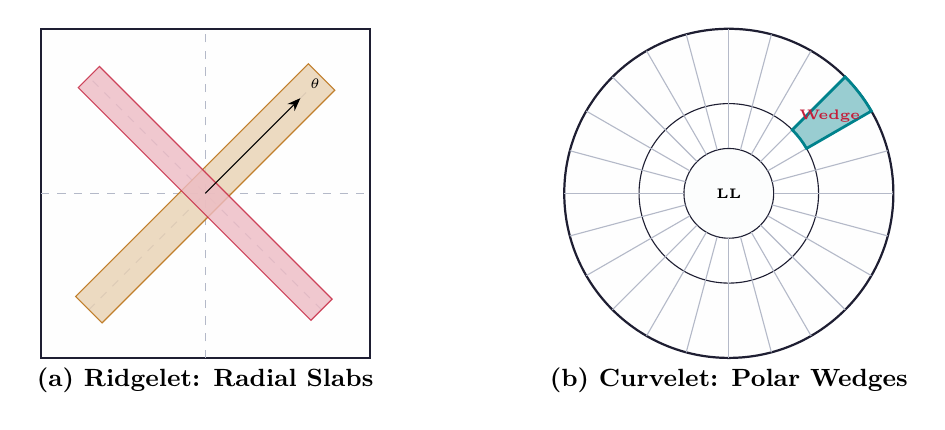
\begin{tikzpicture}[scale=0.95]
  % Ridgelet Partitioning
  \begin{scope}[xshift=-3.5cm]
    \draw[draw=mydark, fill=mygray!10, line width=0.8pt] (-2.2,-2.2) rectangle (2.2,2.2);
    % Radial lines
    \foreach \angle in {0, 45, 90, 135} {
      \draw[dashed, mgframe] (\angle:-2.2cm) -- (\angle:2.2cm);
    }
    % Draw radial slabs
    \draw[fill=myamber!30, draw=myamber, opacity=0.8, rotate=45] (-2.2,-0.25) rectangle (2.2,0.25);
    \draw[fill=myred!30, draw=myred, opacity=0.8, rotate=135] (-2.2,-0.2) rectangle (2.2,0.2);
    \node at (0,-2.5) [font=\small\bfseries] {(a) Ridgelet: Radial Slabs};
    \draw[-Stealth, thin] (0,0) -- (45:1.8cm) node[above right, font=\tiny] {$\theta$};
  \end{scope}

  % Curvelet Partitioning
  \begin{scope}[xshift=3.5cm]
    \draw[draw=mydark, fill=mygray!10, line width=0.8pt] (0,0) circle (2.2cm);
    \draw[fill=white, draw=mydark] (0,0) circle (1.2cm);
    \draw[fill=mygray!30, draw=mydark] (0,0) circle (0.6cm);
    
    % Radial divisions
    \foreach \angle in {0, 15, 30, 45, 60, 75, 90, 105, 120, 135, 150, 165, 180, 195, 210, 225, 240, 255, 270, 285, 300, 315, 330, 345} {
      \draw[mgframe, thin] (\angle:0.6cm) -- (\angle:2.2cm);
    }
    
    % Highlight one Curvelet wedge (Parabolic scaling: length = r*dtheta, width = dr)
    \draw[fill=myteal!40, draw=myteal, line width=1pt] (30:1.2cm) arc (30:45:1.2cm) -- (45:2.2cm) arc (45:30:2.2cm) -- cycle;
    \node[font=\tiny\bfseries, color=myred] at (37.5:1.7cm) {Wedge};
    
    \node at (0,-2.5) [font=\small\bfseries] {(b) Curvelet: Polar Wedges};
    \node at (0,0) [font=\tiny\bfseries] {LL};
  \end{scope}
\end{tikzpicture}
\end{tcolorbox}

% ===============================================================================
\section{Properties and Applications of Ridgelets and Curvelets}
% ===============================================================================

\begin{itemize}[leftmargin=*, itemsep=4.5pt]
  \item \textbf{Properties:} 
        \begin{itemize}[leftmargin=*, itemsep=2.5pt, topsep=2pt]
          \item \textbf{High Directional Sensitivity:} Support orientations increase at finer scales.
          \item \textbf{Optimal Sparsity:} Curvelets represent curved edges with very few non-zero coefficients compared to wavelets.
        \end{itemize}
  \item \textbf{Applications:}
        \begin{itemize}[leftmargin=*, itemsep=2.5pt, topsep=2pt]
          \item \textbf{Seismic Data Processing:} Identifying straight and curved geological faults.
          \item \textbf{CT/MRI Reconstruction:} Solving tomographic reconstruction problems from radon projections.
          \item \textbf{Directional Image Denoising:} Removing noise while preserving sharp curved edges.
        \end{itemize}
\end{itemize}

\newpage
% ===============================================================================
\begin{center}
  {\large\bfseries\color{myred} Quick Revision --- Module 7}\\[3pt]
  {\small\color{mydark} Beyond Wavelet $|$ PE-EC703C}
\end{center}
\noindent{\color{myred}\rule{\linewidth}{1.2pt}}
\vspace{4pt}
% ===============================================================================

\begin{tcolorbox}[formulabox, title={\textbf{Key Equations}}]
\renewcommand{\arraystretch}{1.35}
\begin{tabularx}{\linewidth}{B{5.0cm} X}
Ridgelet Transform & $\psi_{a,b,\theta}(x, y) = a^{-1/2} \psi\left(\frac{x \cos\theta + y \sin\theta - b}{a}\right)$ \\[12pt]
Parabolic Scaling Law & $\text{width} \approx \text{length}^2 \implies \text{width} \propto 2^{-j}, \; \text{length} \propto 2^{-j/2}$
\end{tabularx}
\tcbset{after={\color{black}}}
\end{tcolorbox}

\begin{tcolorbox}[defbox, title={\textbf{One-Line Definitions}}]
\begin{itemize}[leftmargin=*, itemsep=3.5pt]
  \item \textbf{Anisotropic:} Having properties that differ depending on the direction of measurement (e.g., curvelet shape).
  \item \textbf{Radon Transform:} Mathematical integral projection mapping line integrals of a 2D function into 1D profiles.
  \item \textbf{Ridgelet Transform:} Directional 2D transform mapping straight line singularities to point-like representations.
  \item \textbf{Curvelet Transform:} Directional multiscale transform optimized for curved edge singularities.
  \item \textbf{Wrapping Algorithm:} Fast discrete curvelet transform that wraps Fourier wedges into a rectangular grid.
  \item \textbf{USFFT Algorithm:} Fast discrete curvelet transform that uses unequally spaced fast Fourier projections.
\end{itemize}
\end{tcolorbox}

\begin{tcolorbox}[exambox, title={\textbf{Frequently Asked / Viva Questions}}]
\begin{enumerate}[topsep=0pt, label=\textbf{Q\arabic*.}, itemsep=5pt]
  \item \Q{Why are standard wavelets inefficient at representing curved edges in 2D?}
        Separable 2D wavelets have square spatial support. Representing a smooth curved edge requires many small wavelets along the curve at fine scales, which destroys sparsity.

  \item \Q{How is the Ridgelet transform implemented using the Radon transform?}
        The Ridgelet transform is implemented by first applying the Radon transform to project line integrations into 1D profiles, followed by a 1D continuous wavelet transform along those radial profiles.

  \item \Q{What is the parabolic scaling property of curvelets?}
        Curvelets scale such that $\text{width} \approx \text{length}^2$ (i.e. at scale $2^{-j}$, the width is $2^{-j}$ and length is $2^{-j/2}$). This anisotropic, needle-like shape allows curvelets to trace curved edges efficiently.

  \item \Q{Explain the two primary digital curvelet transform algorithms.}
        \begin{itemize}[leftmargin=*, itemsep=1pt, topsep=2pt]
          \item \textbf{USFFT:} Computes spatial coordinates on an irregular polar-like grid in the frequency domain.
          \item \textbf{Wrapping:} Wraps rectangular frequency wedges into a standard rectangular grid to allow fast FFT processing.
        \end{itemize}

  \item \Q{What are the primary applications of Ridgelets and Curvelets?}
        They are used in seismic data processing, CT/MRI tomographic reconstruction, and denoising of images with dominant curved structures, where wavelets would blur the edges.
\end{enumerate}
\end{tcolorbox}

\begin{tcolorbox}[tikzbox, title={\textbf{Multi-Resolution Feature Representation Comparison}}]
\par\noindent
{\renewcommand{\arraystretch}{1.45}%
\begin{tabularx}{\linewidth}{|B{3.0cm}|Y|Y|Y|}
\hline
\textbf{Property} & \textbf{Wavelet Transform} & \textbf{Ridgelet Transform} & \textbf{Curvelet Transform} \\
\hline
\textbf{Dimension} & 1D, 2D, or Multi-D. & 2D (or higher). & 2D (or higher). \\
\hline
\textbf{Optimal For} & Point singularities. & Straight line singularities. & Curved singularities (edges). \\
\hline
\textbf{Support Geometry} & Isotropic (square). & Line-like (infinite slabs). & Needle-like (parabolic wedges). \\
\hline
\textbf{Directionality} & 3 fixed directions in 2D. & Continuous angle $\theta$. & Multi-directional (scale-dependent). \\
\hline
\textbf{Fourier Tiling} & Concentric dyadic squares. & Radial strips. & Polar-like wedges. \\
\hline
\end{tabularx}}
\end{tcolorbox}

\end{document}
